\section{The general minimum makespan parallel motion planning problem on a grid is NP-hard}

\cite{siamcomp/DemaineFKMS19} \cite{corr/YuL15c}

\subsection{Preliminaries}

A (deterministic) \emph{Turing Machine} (TM) is a mathematically modeled machine capable of general purpose computations operating on a tape of symbols. It is generally considered to be equivalent in capabilities to most mathematical definitions of computation \cite{aw/HopcroftU79}. See \cite{aw/HopcroftU79} for a formal definition.

Let a computational problem asking a yes/no question based on some input be called a \emph{decision problem}.

There are different \emph{classes} of computational problems in terms of computational complexity. The \emph{P}-class of problems is defined as the set of decision problems solvable by a TM in \emph{polynomial time}, i.e. in \ilmath{O(n^k)} time on the size of the input \emph{n} and some constant \emph{k}.

The \emph{NP}-class of problems is defined as the set of decision problems that are \emph{verifiable} by a TM in polynomial time. Actually finding a solution to an NP-problem might take considerably longer. It remains an important open question whether P is or is not equal to NP, but many believe P is a proper subset of NP.

A transformation of a problem \ilmath{B} into another problem \ilmath{A} such that a solution to \ilmath{A} solves \ilmath{B} is called a \emph{reduction} and is commonly denoted \ilmath{B \leq A}. If the reduction can be done in polynomial time, it can be denoted \ilmath{B \leq_p A}.

\begin{definition}\label{def:np_complete}
	A decision problem \emph{A} is \emph{NP-complete} (\ilmath{A \in \text{NPC}}) if and only if \emph{A} is in NP and there exists a polynomial time reduction from every problem in NP to \emph{A}:
	\begin{align*}
		A \in \text{NPC} \Leftrightarrow \parens{A \in \NP} \land \parens{B \leq_p A, \; \forall B \in \NP}
	\end{align*}
	NP-complete is essentially the hardest class of problems that can be verified in polynomial time. 
\end{definition}

\begin{remark}\label{rem:p_np_disjoint}
	If \ilmath{\pclass \neq \NP} holds, the classes of P and NP-complete problems are disjoint. Otherwise \emph{all} problems in NP would be polynomially reducible to problems solvable in polynomial time, thus also solvable themselves in polynomial time. This would imply P = NP:
	\begin{align*}
		& \pclass \cap \text{NPC} \neq \emptyset \\
		\Rightarrow \; & \exists A \in \pclass : B \leq_p A, \; \forall B \in \NP \\
		\Rightarrow \; & B \in \pclass, \; \forall B \in \NP \\
		\Rightarrow \; & \pclass = \NP
	\end{align*}
\end{remark}

\begin{definition}\label{def:np_hard}
	A problem \emph{H} is classified as \emph{NP-hard} if there exists a polynomial time reduction \ilmath{A \leq_p H, \; \forall A \in \NP}. Note that \ilmath{H} begin NP-hard does \emph{not} imply \ilmath{H \in \NP}. Though if \ilmath{H} can be proven to belong to NP, i.e. be verifiable in polynomial time, \ilmath{H} will then by definition be NP-complete.
\end{definition}

	% Note:
	% \begin{align*}
	% 	H \in \NP \Rightarrow H \text{ is NP-hard} \\
	% 	H \text{ is NP-hard} \not\Rightarrow H \in \NP
	% \end{align*}
\begin{remark}\label{rem:p_np_hard_disjoint}
	The same construction as in \cref{rem:p_np_disjoint} works here too, P and NP-hard problems are disjoint, assuming \ilmath{\pclass \neq \NP}.
\end{remark}

\begin{remark}\label{note:npc_proving}
	Let \ilmath{A} be some known NP-complete problem. If there is a polynomial time reduction from \ilmath{A} to some other problem \ilmath{B}: \ilmath{A \leq_p B}, we know that \ilmath{B} is NP-hard. Further proving that \ilmath{B} is NP-complete would require \emph{either} a polynomial reduction from \ilmath{B} to \ilmath{A}: \ilmath{B \leq_p A} \emph{or}, possibly easier, proving that \ilmath{B} is in NP; proving that \ilmath{B} is deterministically verifiable in polynomial time.
\end{remark}

Let a \emph{boolean expression} be composed of boolean variables \ilmath{b \in \set{\true,\, \false}}, negations (\texttt{not } \ilmath{\neg}), conjunctions (\texttt{and} \ilmath{\land}), disjunctions (\texttt{or} \ilmath{\lor}) and parentheses.

The following is an example of a boolean expression:
\begin{align}\label{ex:boolean_xor}
	\parens{b_1 \lor b_2} \land \neg \parens{b_1 \land b_2}
\end{align}

Let a \emph{literal} be a variable \ilmath{b} (a positive literal) or the negation of a variable \ilmath{\neg b} (a negative literal). A (disjunctive) \emph{clause} is then defined as a disjunction of literals \ilmath{C = \parens{l_1 \lor l_2 \lor \dots \lor l_k}, \ l_i \in \set{b_j,\ \neg b_j}}. 

Let a boolean expression be in \emph{Conjunctive Normal Form} (CNF) if and only if it is composed only of adjunctions of disjunctive clauses. The previous example in \cref{ex:boolean_xor} is \emph{not} in CNF, as negation of a clause is not allowed, and the second parenthesis is an adjunction, not a disjunction.

\begin{remark}
	It is always possible, but non-trivial, to transform an arbitrary boolean expression into CNF \cite{?}. The expression in \cref{ex:boolean_xor} can be stated in CNF as follows:
	\begin{align}\label{ex:cnf_xor}
		\parens{b_1 \lor b_2} \land \parens{\neg b_1 \lor \neg b_2}
	\end{align}
\end{remark}

Let \ilmath{\varphi} be a boolean expression in Conjunctive Normal Form. The boolean satisfiability problem, abbreviated \emph{SAT}, is a decision problems asking whether \ilmath{\varphi} can be evaluated to \true\ for some state of its variables \ilmath{\set{b_1, b_2, \dots, b_n} \in \set{\true, \false}^{n}}. It is trivial to verify if a solution is correct or not: a boolean expression can be evaluated well within polynomial time, thus SAT has to be in NP. On the other hand, there are an exponential amount of states of the input variables: \ilmath{2^n} states for the \ilmath{n} input variables to be exact. It has been proven that SAT is NP-complete, and a sub-exponential algorithm for solving a general SAT problem would indeed be groundbraking. 

The corresponding SAT problem to \cref{ex:cnf_xor} would ask whether it is satisfiable. This particular expression is satisfiable, as when \ilmath{\coord{b_1}{b_2} = (\true, \false)} or \ilmath{\coord{b_1}{b_2} = \coord{\false}{\true}} the expression evaluates to \true, coincidentally equivalent to an \texttt{xor}\ expression.

\begin{definition}
	Let \emph{3SAT} be a subset of SAT, such that any problem in 3SAT has exactly 3 literals in each clause. 3SAT is also known to be NP-complete.
\end{definition}

\begin{definition}
	A \emph{Monotone 3SAT} is defined as a further restricted version of 3SAT, such that each clause of the expression has all-positive or all-negative literals. 
\end{definition}

% Boolean expressions are constructed from positive and negative literals (\ilmath{x} and \ilmath{\neg x} respectively), conjunctions (AND \ilmath{\land}), disjunctions (OR \ilmath{\lor}) and parentheses. An example SAT problem would ask whether \ilmath{}


\subsection{The theorem}

\note{should this be in preliminaries?}

Let a decision problem formulation of minimum makespan motion planning be as follows: Given start and end configurations \ilmath{\conf{s}} and \ilmath{\conf{t}} respectively, is there a schedule that can transform \ilmath{\conf{s} \rightarrow \conf{t}} with makespan at most \emph{M}? 

\begin{lemma}\label{lemma:np}
	The decision problem formulation of a minimum makespan motion planning problem is in NP.
\end{lemma}

\begin{proof}
	It is also easy to show that the decision problem is in NP; to verify a solution, one has to check three things:
	\begin{enumerate}
		\item Every transformation step of a schedule should be valid according to \cref{req:limited_movement} and \cref{req:no_swaps}.\label{checks:transformations}
		\item After the last step of execution, the configuration should equal that of \ilmath{\conf{t}}.\label{checks:target_acquired}
		\item There should be at most \ilmath{M} transformation steps.\label{checks:makespan}
	\end{enumerate}
	\cref{req:limited_movement} can be checked in linear time with respect to the robots for each timestep. \cref{req:no_swaps} will need to be checked for each single-robot move, which is bounded by the number of robots for each timestep. Thus \cref{checks:transformations} can be checked in \ilmath{O(m\cdot n)} time, where \ilmath{m} is the makespan and \ilmath{n} is the number of robots. \cref{checks:target_acquired} can be done linearly with respect to the number of robots, as checking the positions for every robot is sufficient (configurations are assumed to be valid, and that \ilmath{\iconf{}{r}} would raise an error if the mapped position would not be deterministically defined). Trivially \cref{checks:makespan} can be done in constant time. 

	A solution is thus verifiable in polynomial time, which implies the problem is in NP by definition.
\end{proof}

\begin{theorem}\label{thm:npc}
	The decision problem formulation of a minimum makespan motion planning problem on a grid is NP-complete.
\end{theorem}

\begin{proof}
	The following proof by \cite{siamcomp/DemaineFKMS19} is done by a polynomial reduction from \emph{Monotone 3SAT} to a decision formulation of a coordinated multi-robot motion planning problem. As Monotone 3SAT is known to be NP-complete, a reduction M. 3SAT \ilmath{\leq_p} M3PP implies M3PP is NP-hard. Together with \cref{lemma:np}, this implies M3PP is also NP-complete. 

	\subsubsection*{The reduction} 
	Let \ilmath{\varphi} be some boolean expression corresponding to some Monotone 3SAT problem. The idea is to construct start and target configurations \ilmath{\conf{s}} and \ilmath{\conf{t}} respectively such that a specific makespan \emph{M} is achievable if and only if the original expression \ilmath{\varphi} is satisfiable, otherwise requiring \ilmath{M + 1} transformation steps at a minimum to transform \ilmath{\conf{s} \rightarrow \conf{t}}.

	% Let our target makespan \emph{M} be fixed at the end of the construction, so that a schedule with makespan \emph{M} is achievable if and only if the original expression \ilmath{\varphi} is satisfiable, otherwise a schedule with makespan \ilmath{M + 1}. 

	The formula \ilmath{\varphi} is composed of \ilmath{n} boolean variables \ilmath{\set{b_1, b_2, \dots, b_n}} and \ilmath{m} clauses \ilmath{\set{C_1, C_2, \dots, C_m}} with three literals each. Let us first represent each variable \ilmath{b_j} with a \emph{variable robot} \ilmath{r_j}.

	Let us consider the path of a single variable robot \ilmath{r_j} first. Let \ilmath{y_j} be the starting \ilmath{y}-coordinate for a specific variable robot \ilmath{r_j} for simplicity, with a definition following later in conjunction with adding multiple variables. Each variable robot starts at the left of our workspace, at \ilmath{ \coord{0}{y_j} }, and has its target position at the right of the workspace, at \ilmath{ \coord{M - 2}{y_j} }. Notice it has two steps to spare relative to a straight path towards the target, and could thus move one step up and one step down \emph{or} wait for up to two timesteps along the way.

	Let there be two \emph{auxiliary robots} for each variable robot, \emph{constraining} the variable robot \ilmath{r_j}: a left auxiliary robot starts at \ilmath{ \coord{1}{y_j + 1} } and has to move down at every timestep towards its goal at \ilmath{ \coord{1}{y_j + 1 - M} }. Similarly, a right auxiliary robot starts at \ilmath{ \coord{M - 3}{y_j + 1 - M} } and moves upwards at every timestep toward its target at \ilmath{ \coord{M - 3}{y_j + 1} }. As a result, the variable robot \ilmath{r_j} is blocked from moving right at timestep 0 by the left auxiliary robot, and is required to be at \ilmath{x = (M - 2)} before timestep \ilmath{M}, otherwise being cut off by the right auxiliary robot.

	The variable robot is then \enquote{free} to \enquote{choose} to either wait at timesteps 0 and \ilmath{M}, traveling at a constant height of \ilmath{y_j} towards its target, or alternatively, moving upwards to \ilmath{y_j + 1} at timestep 0 and down at timestep \ilmath{M}. Let the lower path be equivalent to an assignment of \true\  to \ilmath{b_j}, while the upper path is equivalent to a \false\ assignment to \ilmath{b_j}.

	
\begin{figure}[h]
	\centering
	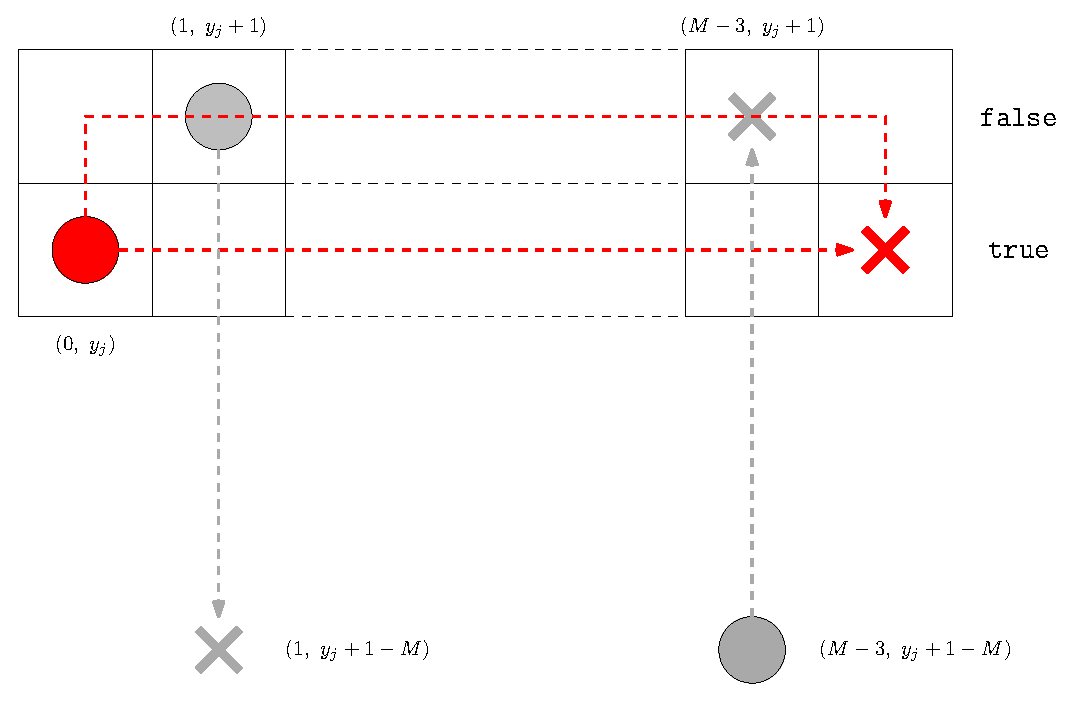
\includegraphics[width=10cm]{ipe/variable_and_first_aux.eps}
	\caption{A minimal example of an unsolvable motion planning problem: there exists no valid schedule which swaps the green and blue robots.}\label{fig:reachability}
\end{figure}

	\note{very WIP here onwards}
	For each clause \ilmath{C_i = \set{ b_{j_1}, b_{j_2}, b_{j_3} }}, let us have three corresponding \emph{checker robots} \ilmath{\set{\checker{1}, \checker{2}, \checker{3}}} checking their respective literal, and one \emph{clause robot} checking that at least one checker robot evaluates to \true\ for that clause. Let each checker robot start diagonally downwards from its respective variable robot, and move in the positive \ilmath{xy}-direction towards its target, across the path of the variable robot. Let it be positioned so that it has to wait for the variable robot for one timestep iff the assignment of the variable robot is mismatched with the literal. 




	If it corresponds to a positive literal, \ilmath{position} otherwise. Let each checker robot have a target position of \ilmath{start + offset}. This means the checker robot has to pass by its corresponding variable robot, and wait for one timestep if and only if the variable assignment is a mismatch with respect to the literal. 

	,  Let their start positions be defined as \ilmath{\alpha_{i_k} \coloneqq}.



	\vdots 

	It is thus possible to reduce \texttt{Monotone 3SAT} into a parallel motion planning problem of finding a minimum makespan, which implies minimum makespan parallel motion planning is NP-hard.
 
\end{proof}

\begin{corollary}
	Computing a minimum makespan schedule for a given motion planning problem is NP-hard.
\end{corollary}

\begin{proof}
	The decision problem formulation of the same problem is shown to be NP-complete. It can trivially be reduced to the problem of finding a minimum makespan schedule, as finding a minimum makespan schedule would solve our decision problem. 
\end{proof}
